\documentclass{article}
\usepackage[icelandic]{babel}
\usepackage[T1]{fontenc}
\usepackage[utf8]{inputenc}


\usepackage{subfig}

\usepackage{todonotes}
\usepackage{color}

%Leitað er af myndum í eftirfarandi möppum
\graphicspath{{./pics/}{../sprettir/}}
\linespread{1.5}

\usepackage{graphicx}
\usepackage{wrapfig}
\usepackage{float}
\usepackage{verbatim}
\usepackage[none]{hyphenat}

\begin{document}
\raggedright

\tableofcontents
\newpage
\section{Kröfulisti}
Kröfulistanum okkar var skipt upp í tvo hluta þar sem verkefninu okkar var skipt upp í tvo fasa. Að neðan er hægt að sjá niðurbrennslurit og kröfulista fyrir báða fasana.

Hér má sjá kröfulistan fyrir verkefnið okkar, kerfið Rýni.

\begin{figure}[H]
  \centering
  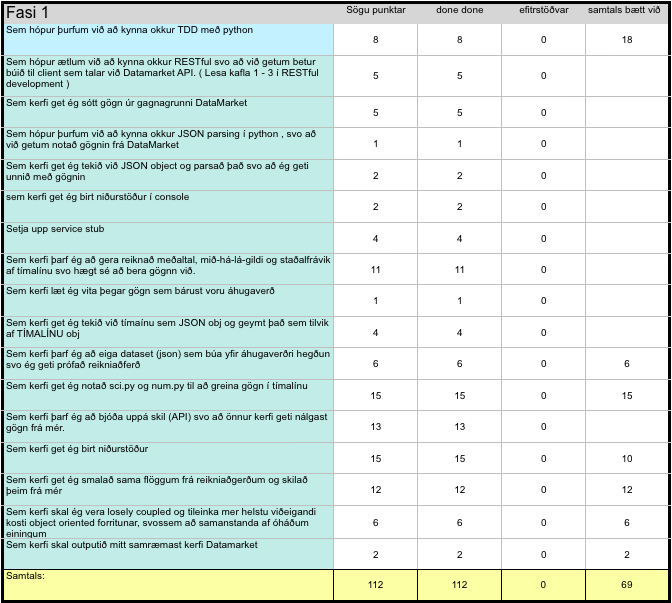
\includegraphics[width=1\textwidth]{Fasi1.png} 
  \caption{Fasi 1} 
\end{figure}

\begin{figure}[H]
  \centering
  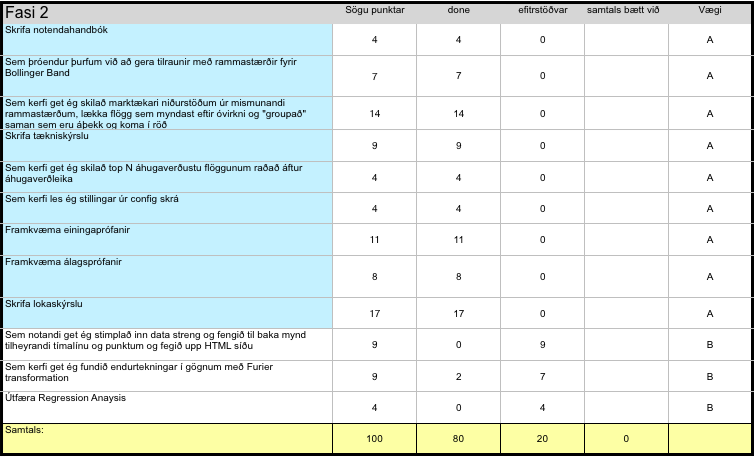
\includegraphics[width=1\textwidth]{Fasi2.png} 
  \caption{Fasi 2} 
\end{figure}

\newpage

\subsection{Burndown}
Hér ber að líta niðurbrennslurit (e. burndown chart) yfir framvindu verkefnisins.

\begin{figure}[H]
  \centering
  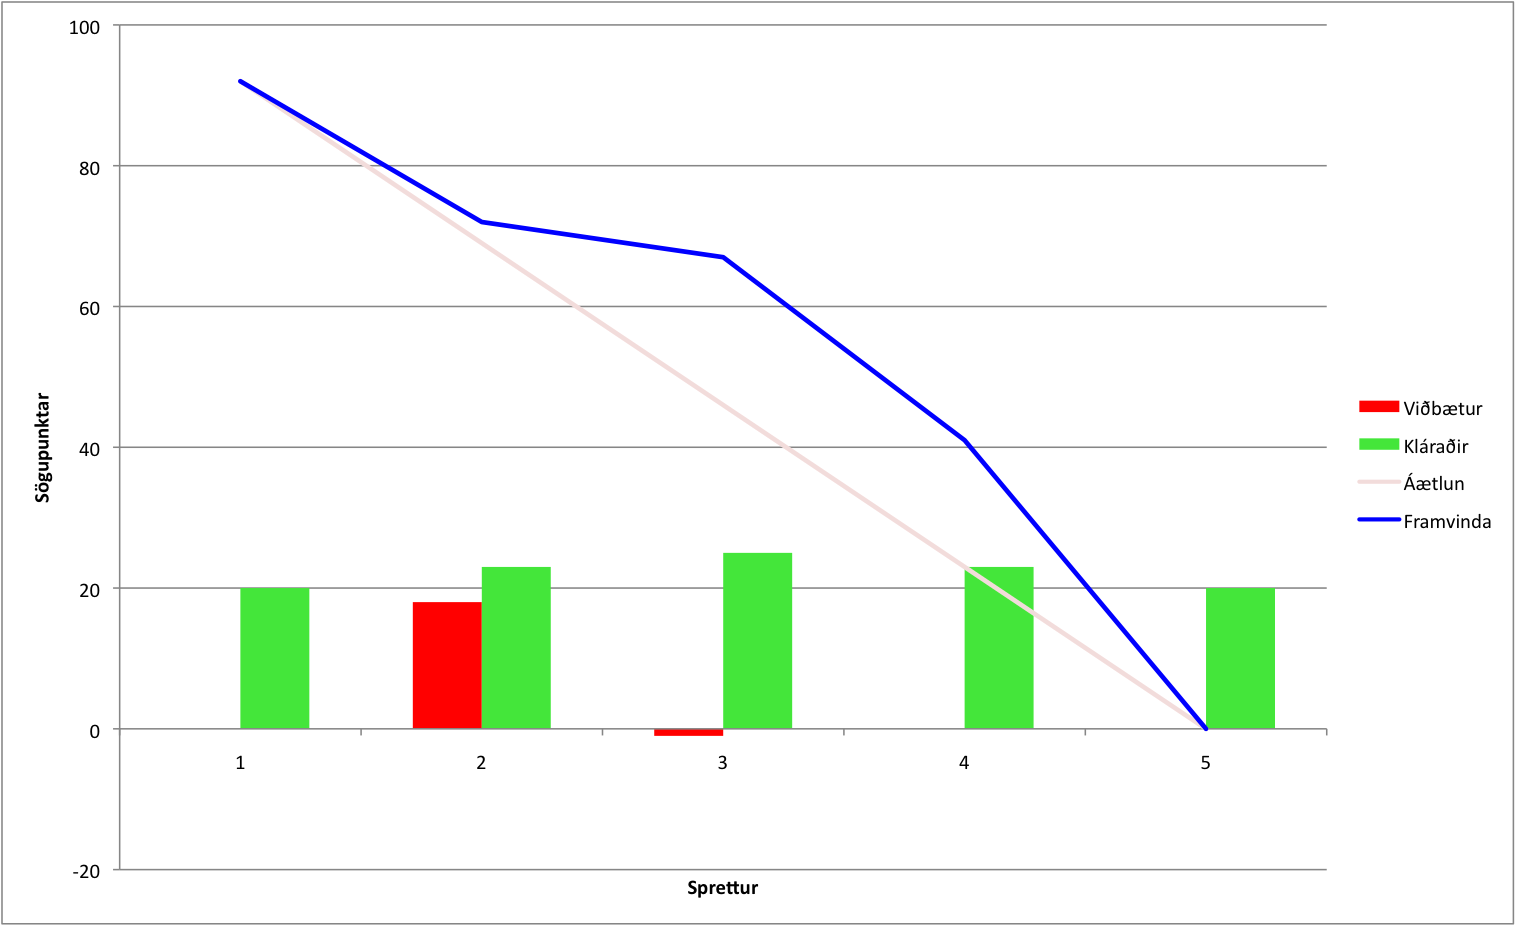
\includegraphics[width=1\textwidth]{Fasi1_burndown.png} 
  \caption{fasi 1} 
\end{figure}

\begin{figure}[H]
  \centering
  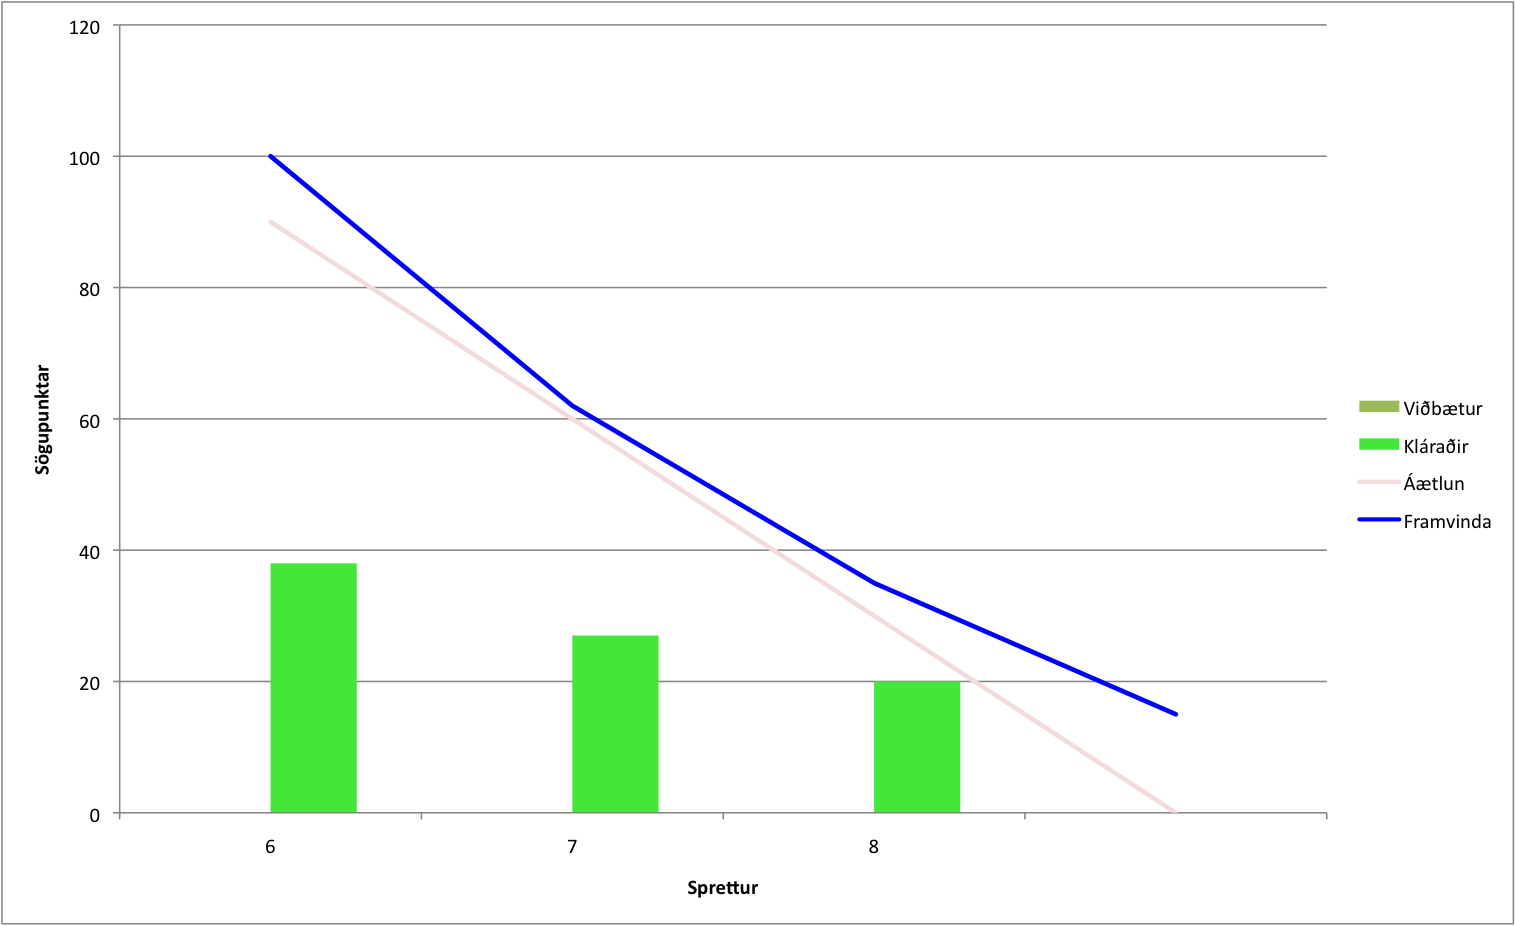
\includegraphics[width=1\textwidth]{Fasi2_burndown.png} 
  \caption{fasi 2} 
\end{figure}

\newpage
\section{Sprettir}
Hér má sjá yfirlitsgröf yfir spretti verkefnisins. Hægt að er sjá sögur og verkliði hvers spretts fyrir sig í meðfylgjandi skjali Sprettir.pdf

\subsection{Sprettur 1}

\begin{figure}[H]
  \centering
  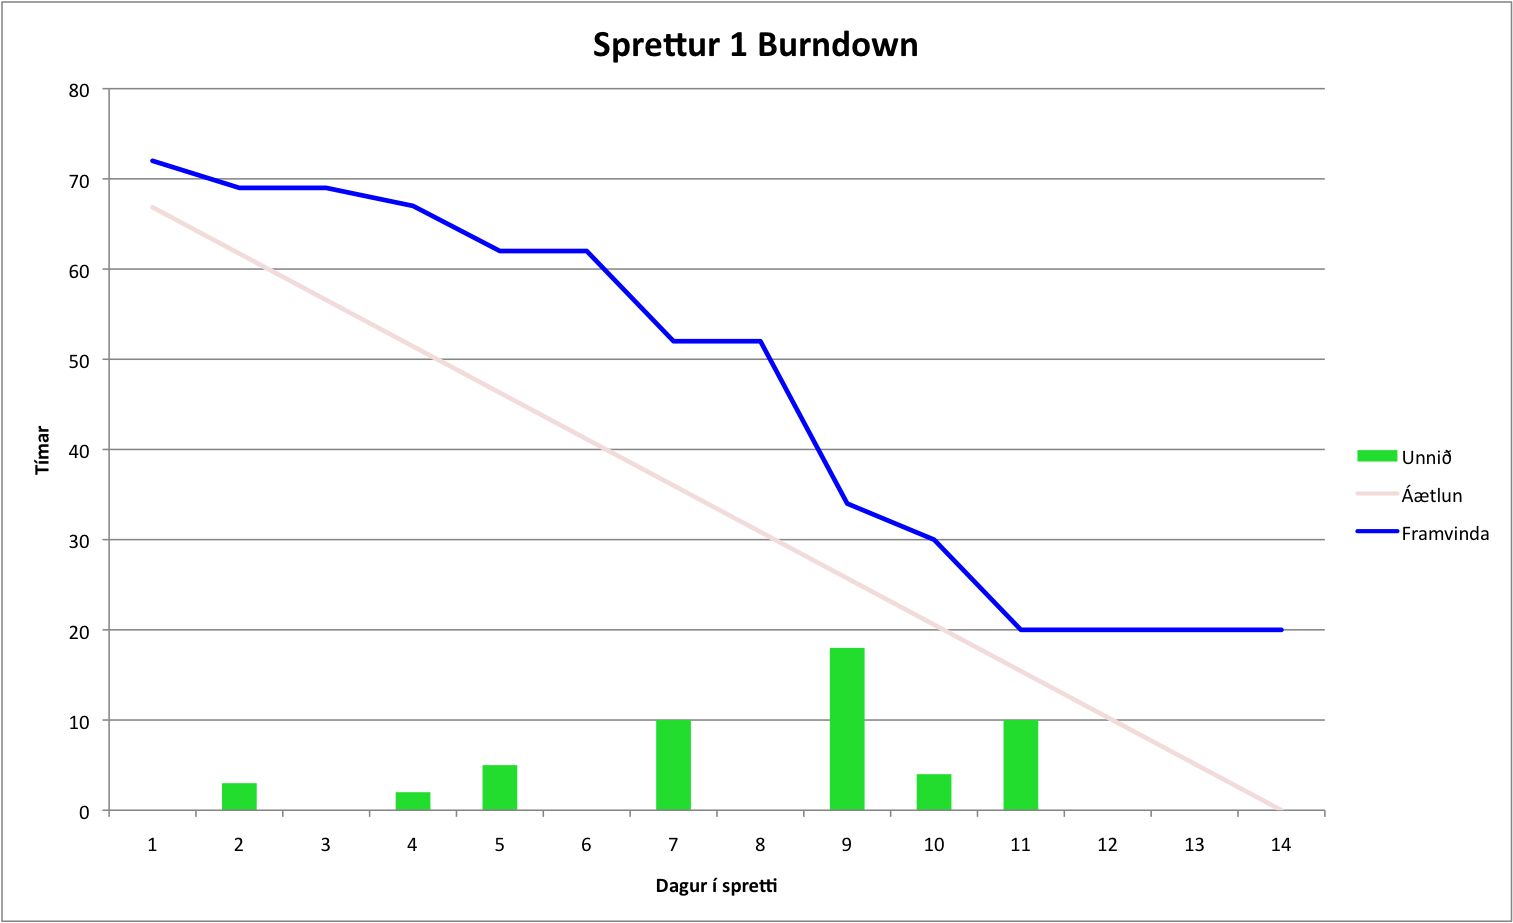
\includegraphics[width=1\textwidth]{Sprettur1_Burndown.png} 
  \caption{Sprettur 1} 
\end{figure}

\subsection{Sprettur 2}

\begin{figure}[H]
  \centering
  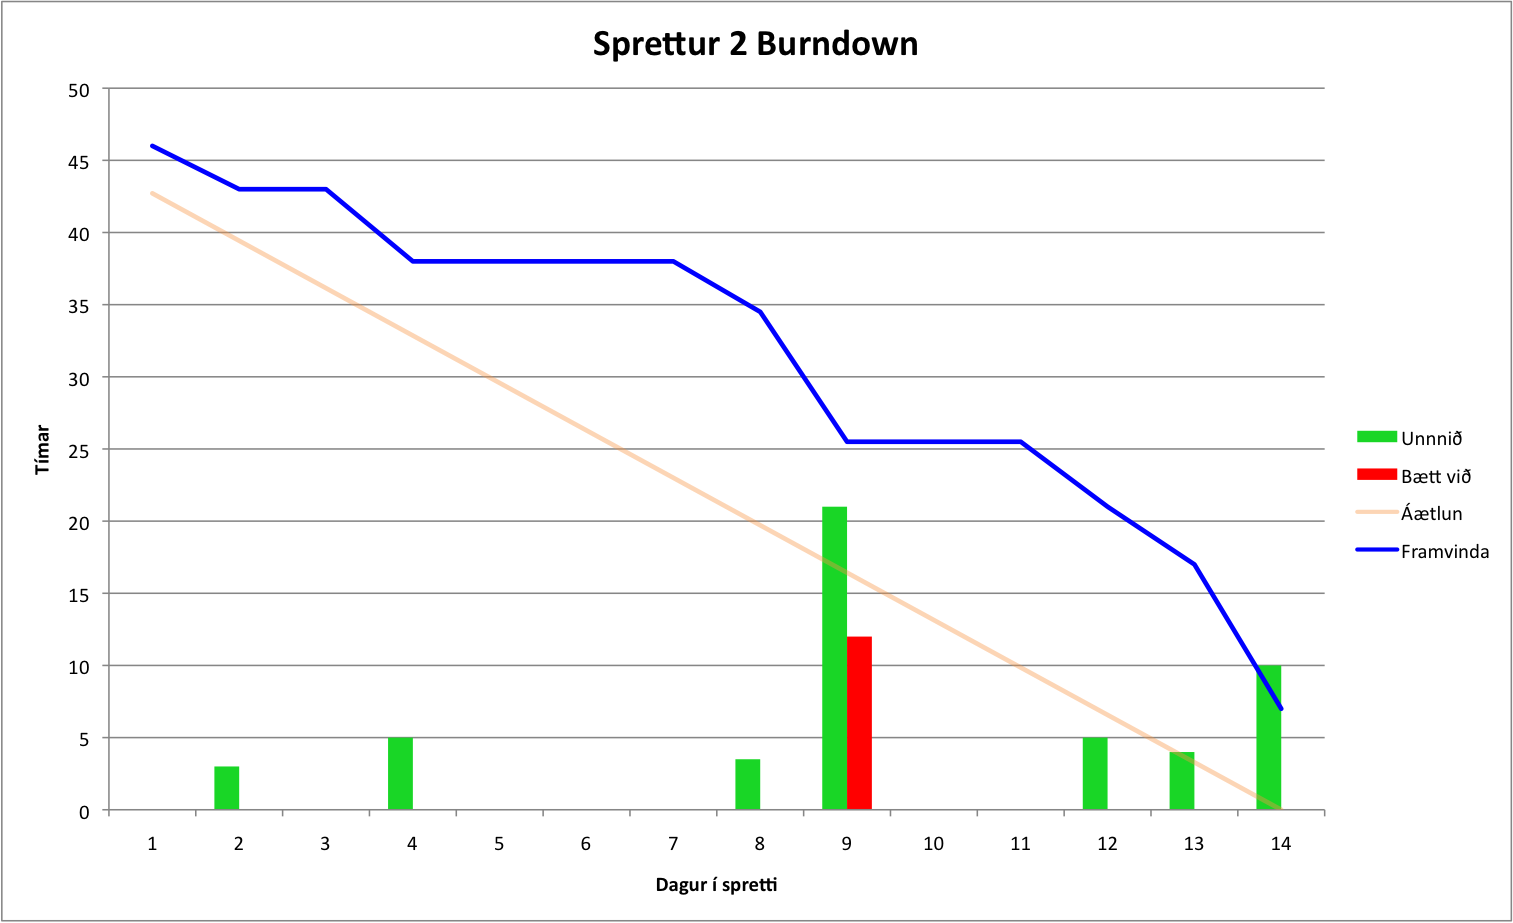
\includegraphics[width=1\textwidth]{Sprettur2_Burndown.png} 
  \caption{Sprettur 2} 
\end{figure}

\subsection{Sprettur 3}

\begin{figure}[H]
  \centering
  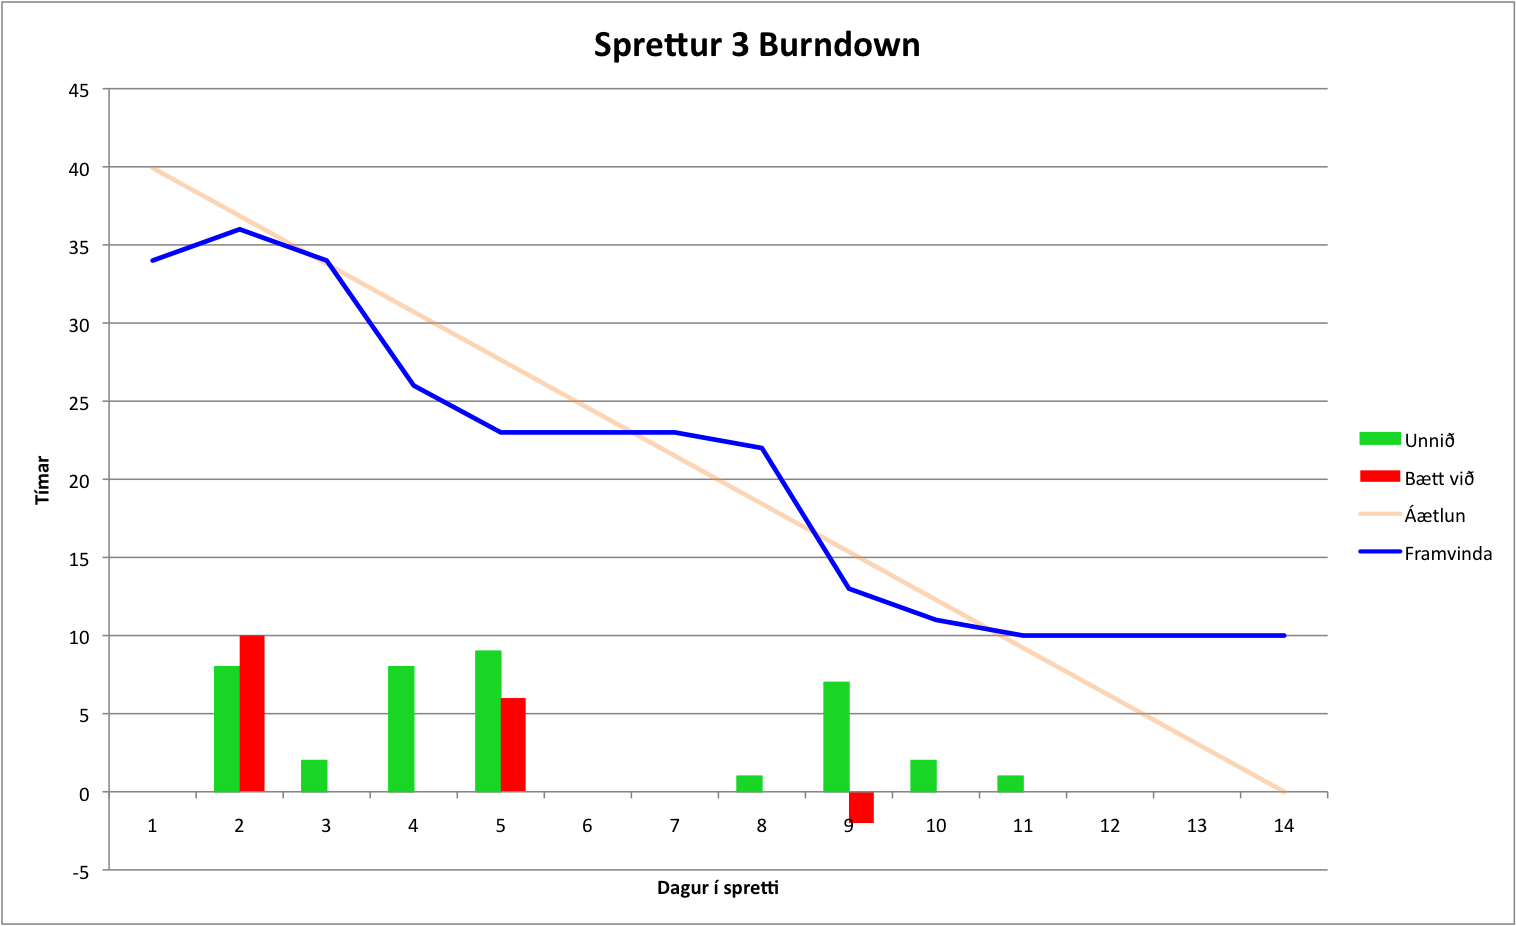
\includegraphics[width=1\textwidth]{Sprettur3_Burndown.png} 
  \caption{Sprettur 3} 
\end{figure}

\subsection{Sprettur 4}

\begin{figure}[H]
  \centering
  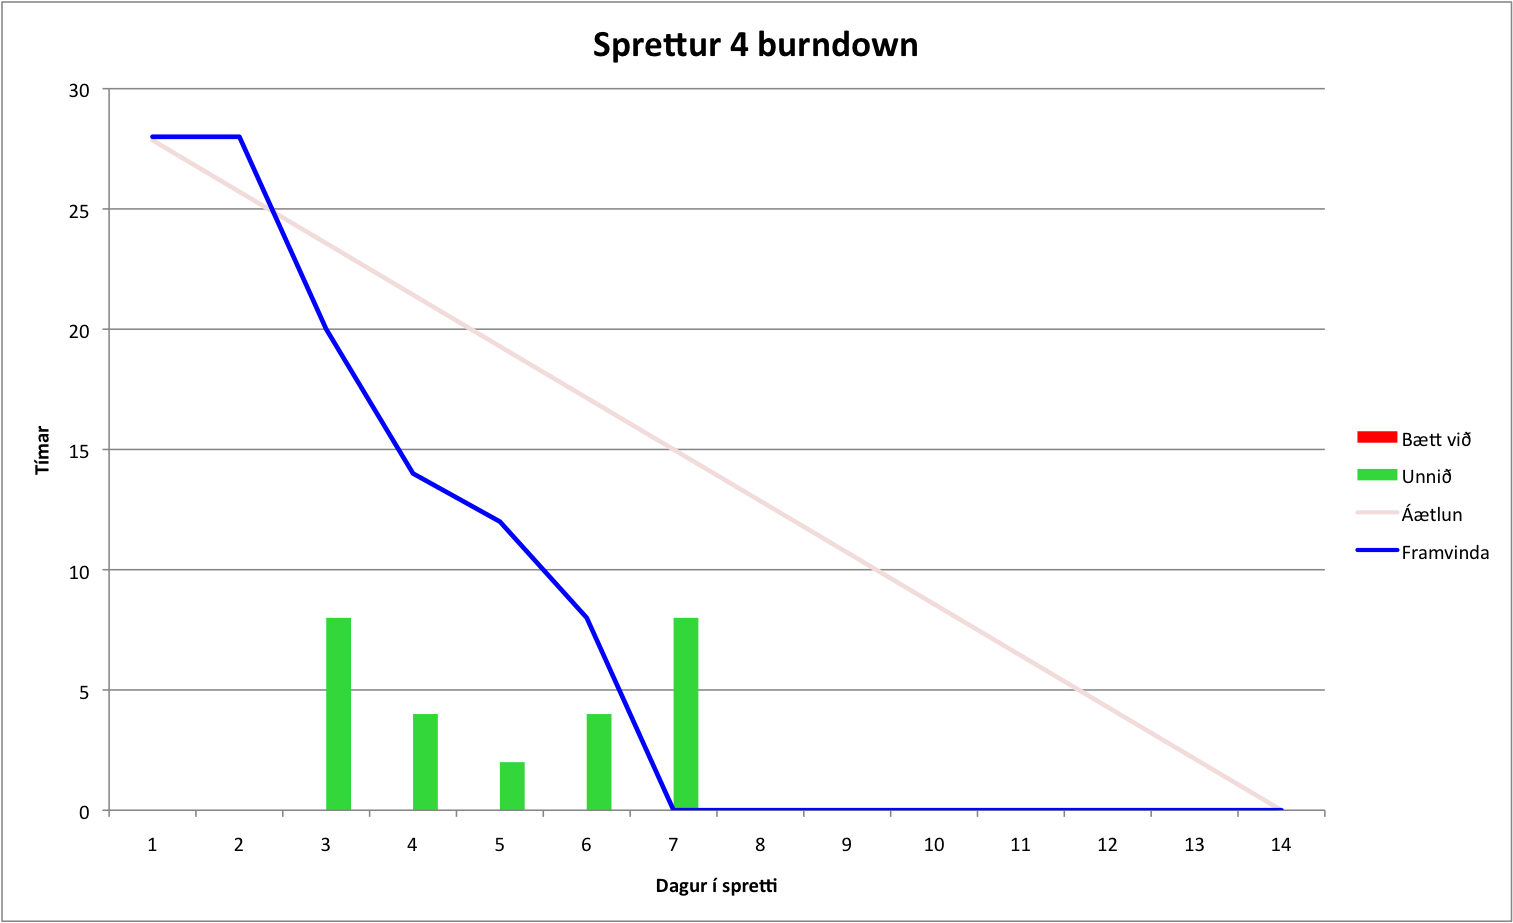
\includegraphics[width=1\textwidth]{Sprettur4_Burndown.png} 
  \caption{Sprettur 4} 
\end{figure}

\subsection{Sprettur 5}

\begin{figure}[H]
  \centering
  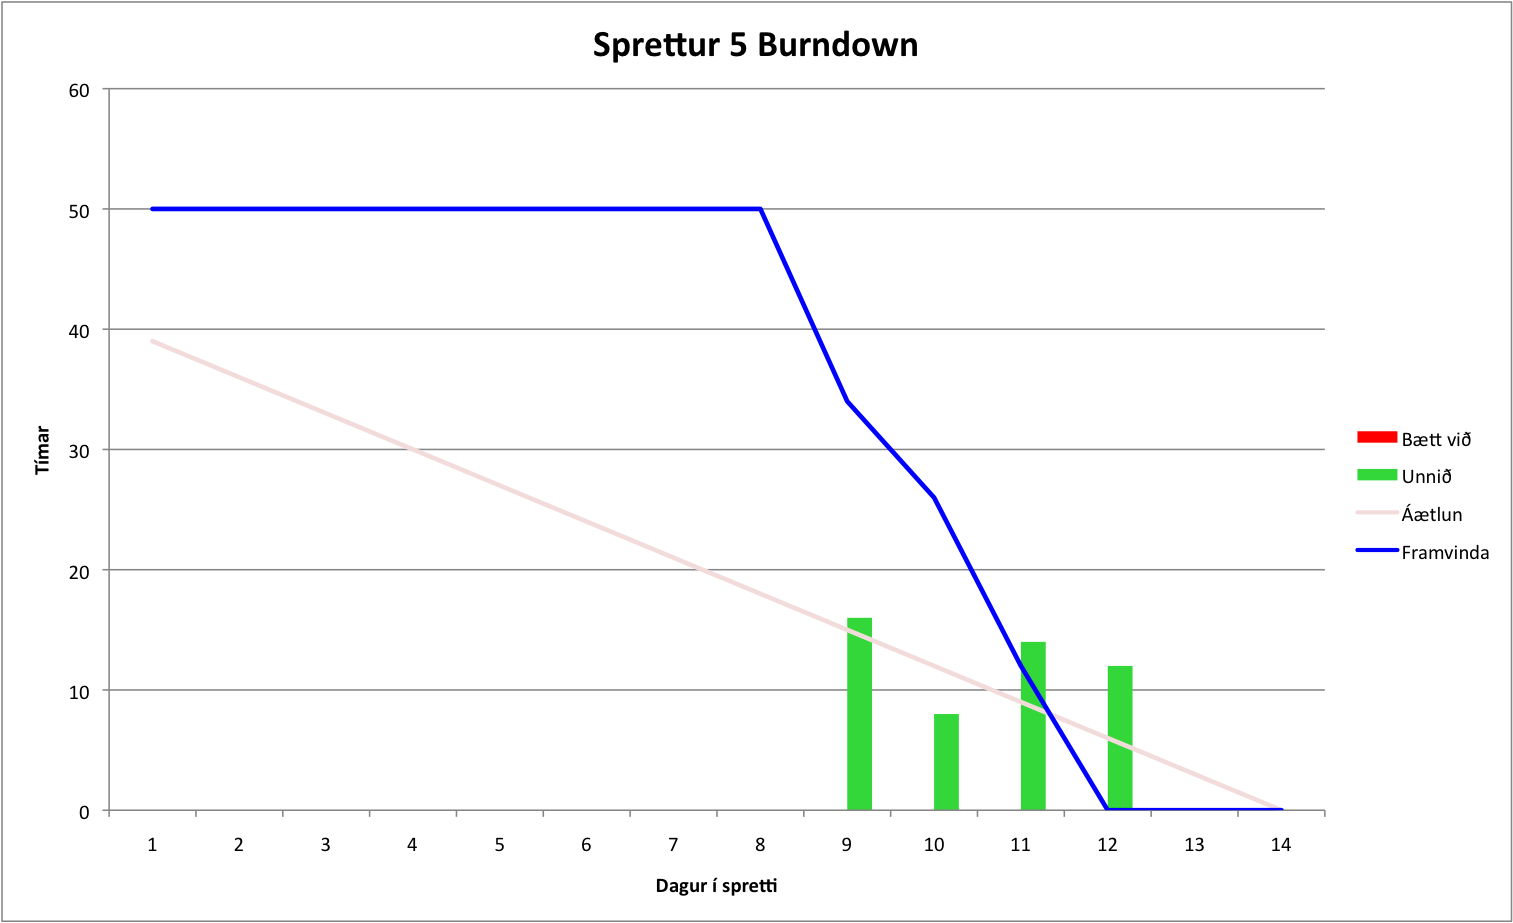
\includegraphics[width=1\textwidth]{Sprettur5_Burndown.png} 
  \caption{Sprettur 5} 
\end{figure}

\subsection{Sprettur 6}

\begin{figure}[H]
  \centering
  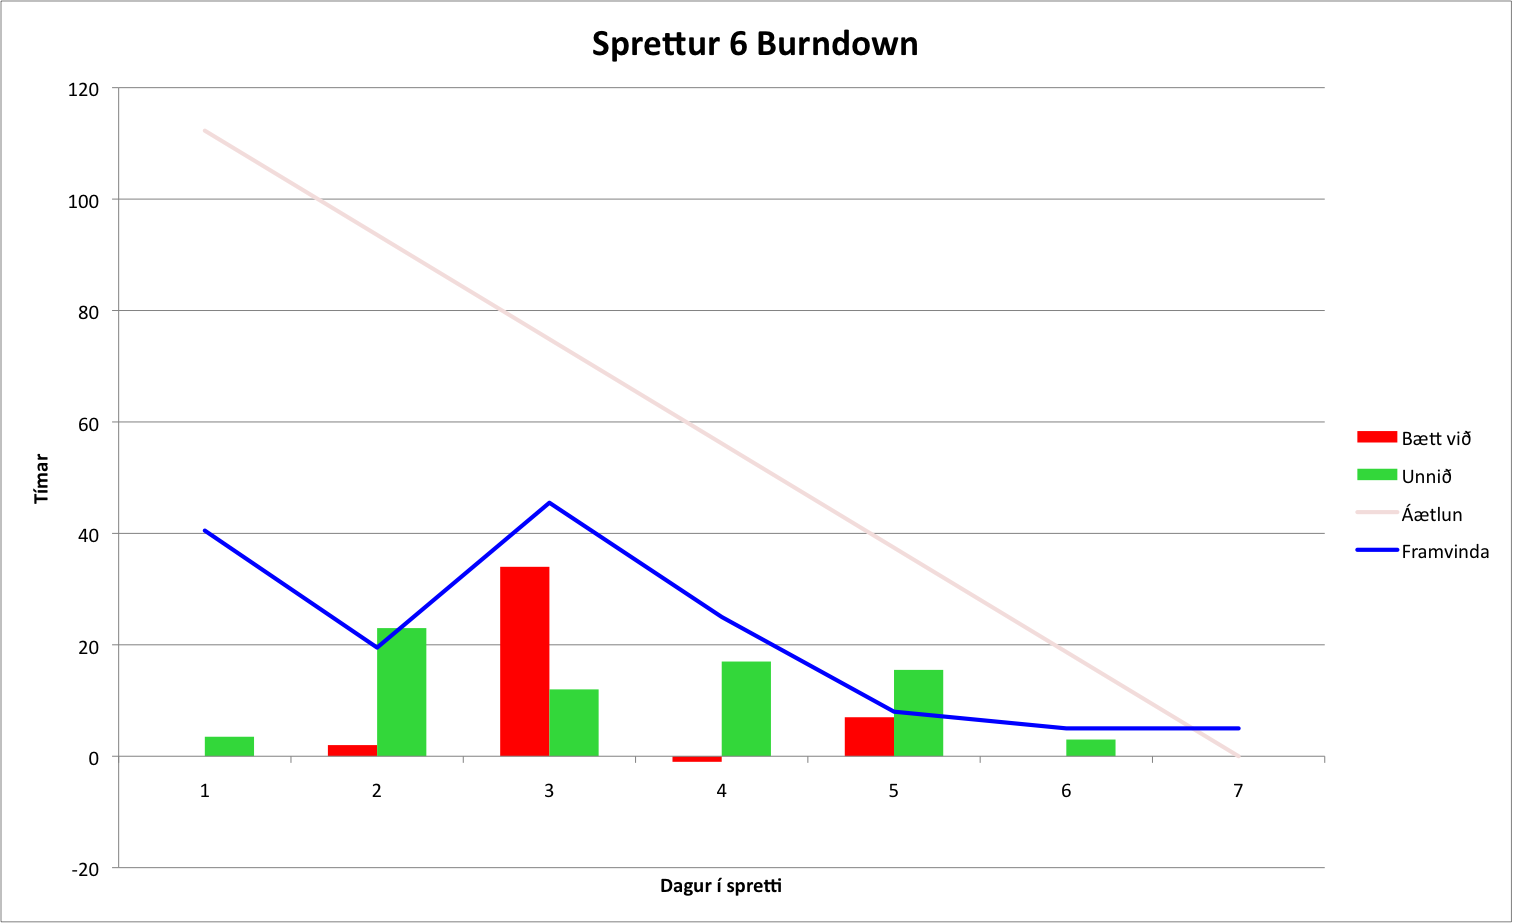
\includegraphics[width=1\textwidth]{Sprettur6_Burndown.png} 
  \caption{Sprettur 6} 
\end{figure}

\subsection{Sprettur 6}

\begin{figure}[H]
  \centering
  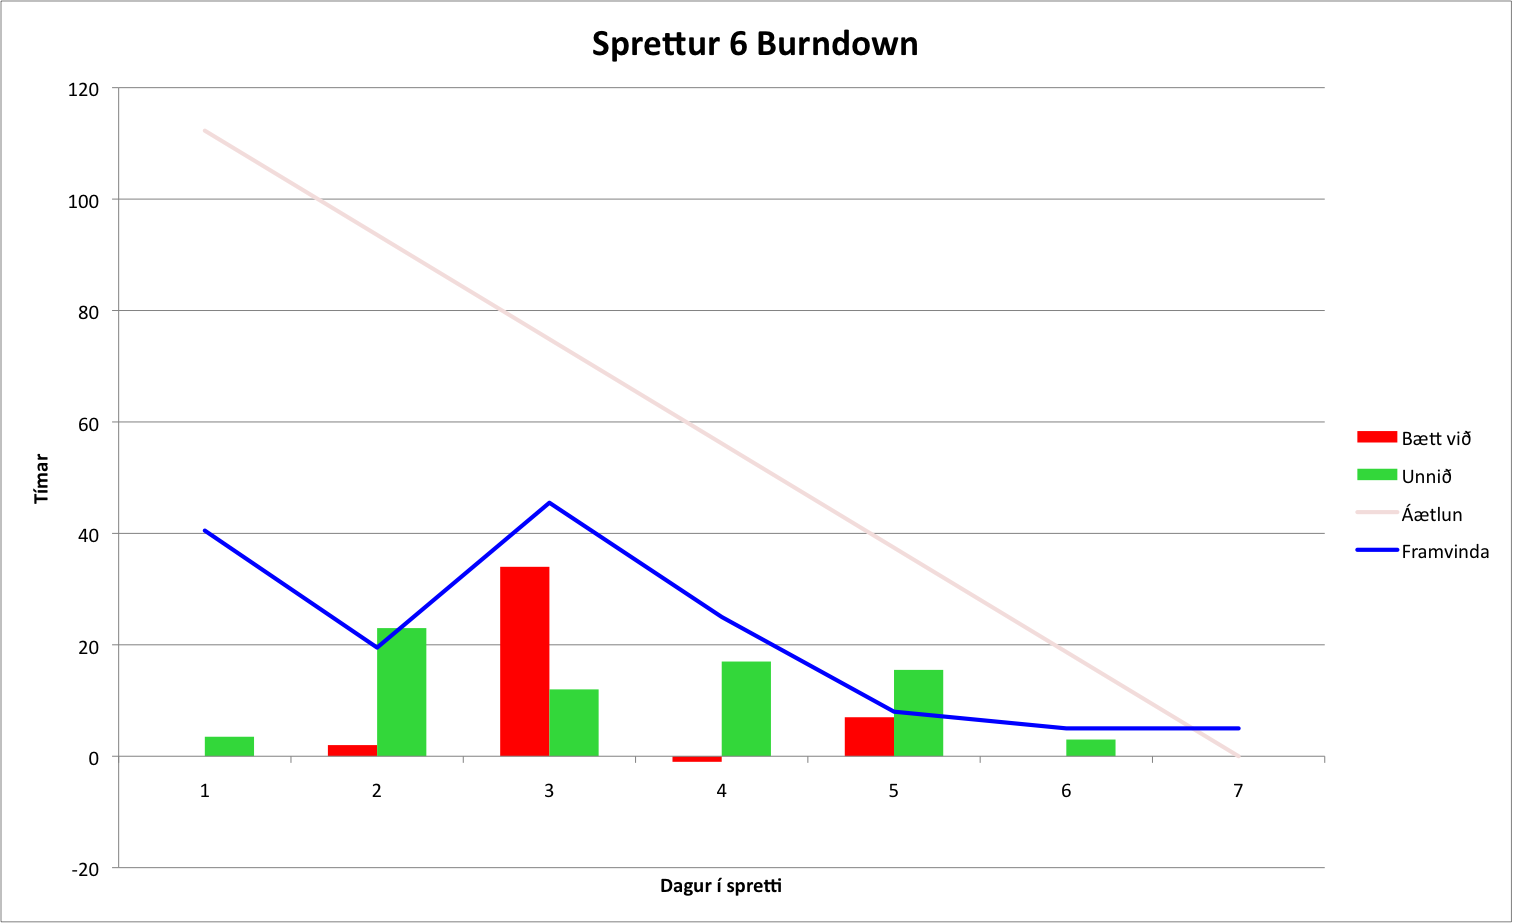
\includegraphics[width=1\textwidth]{Sprettur6_Burndown.png} 
  \caption{Sprettur 6} 
\end{figure}

\subsection{Sprettur 7}

\begin{figure}[H]
  \centering
  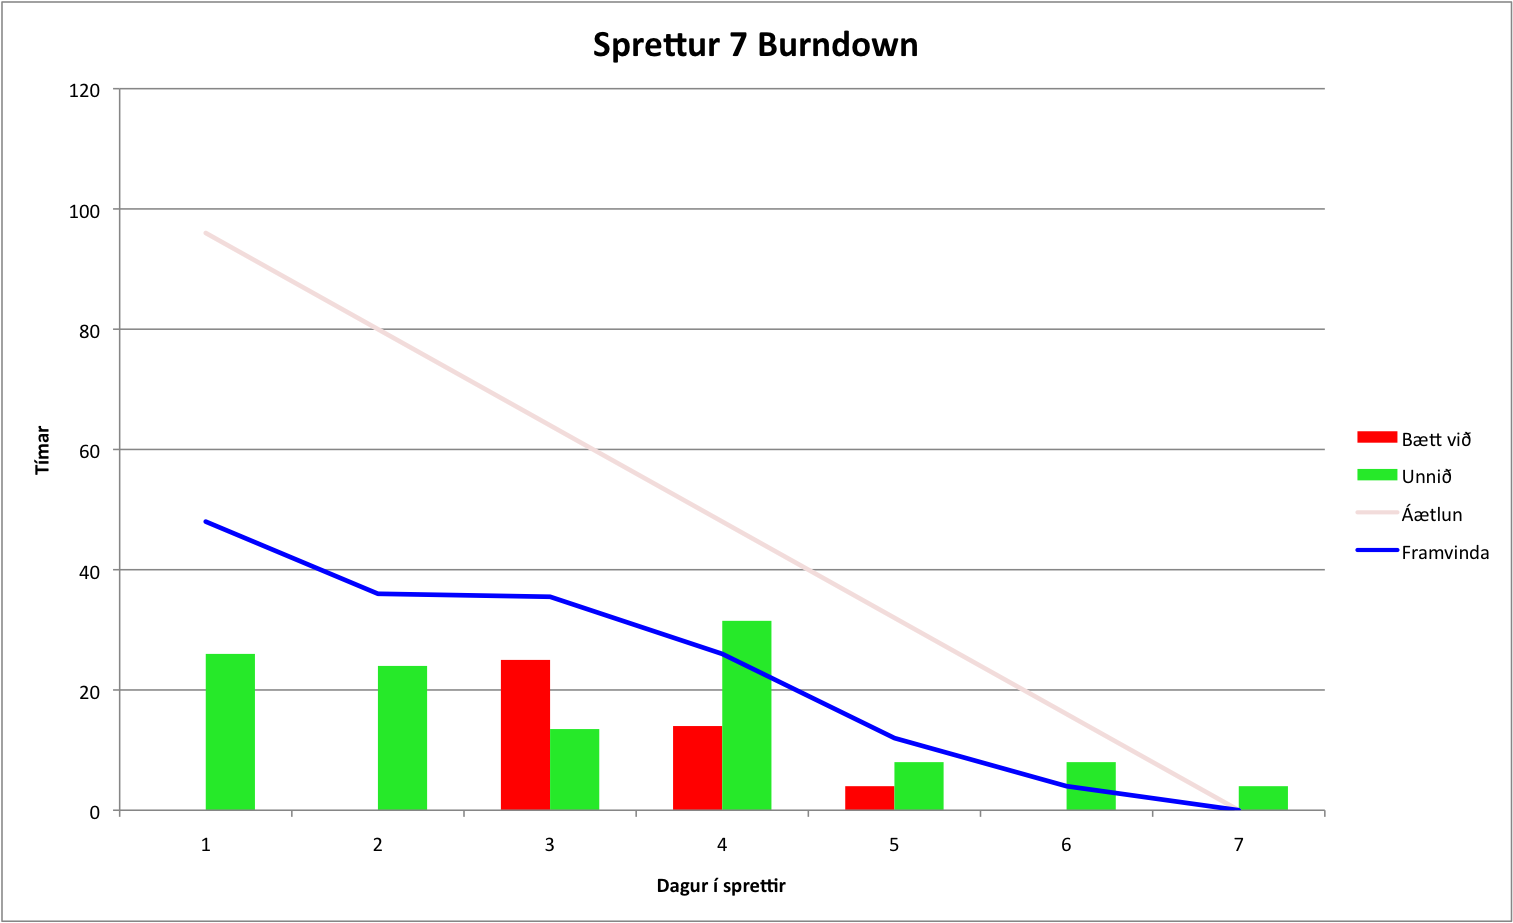
\includegraphics[width=1\textwidth]{Sprettur7_Burndown.png} 
  \caption{Sprettur 7} 
\end{figure}

\subsection{Sprettur 8}

\begin{figure}[H]
  \centering
  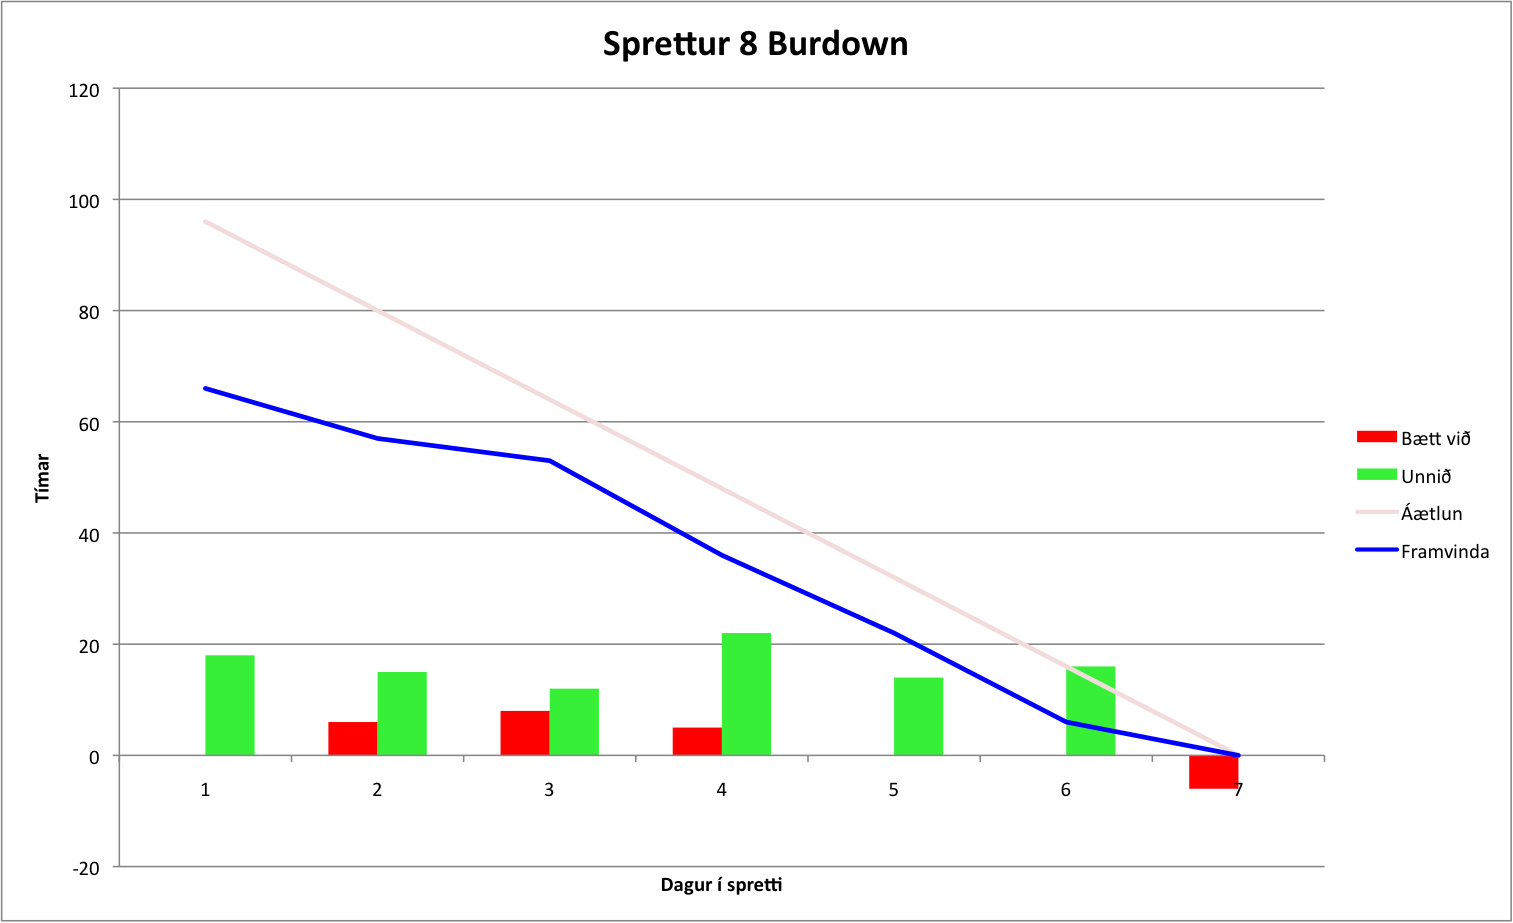
\includegraphics[width=1\textwidth]{Sprettur8_Burndown.png} 
  \caption{Sprettur 8} 
\end{figure}

\newpage
\section{Tímaskráning}
Hér má sjá yfirlit yfir þá tíma sem unnir voru í verkefninu. 

\begin{figure}[H]
  \centering
  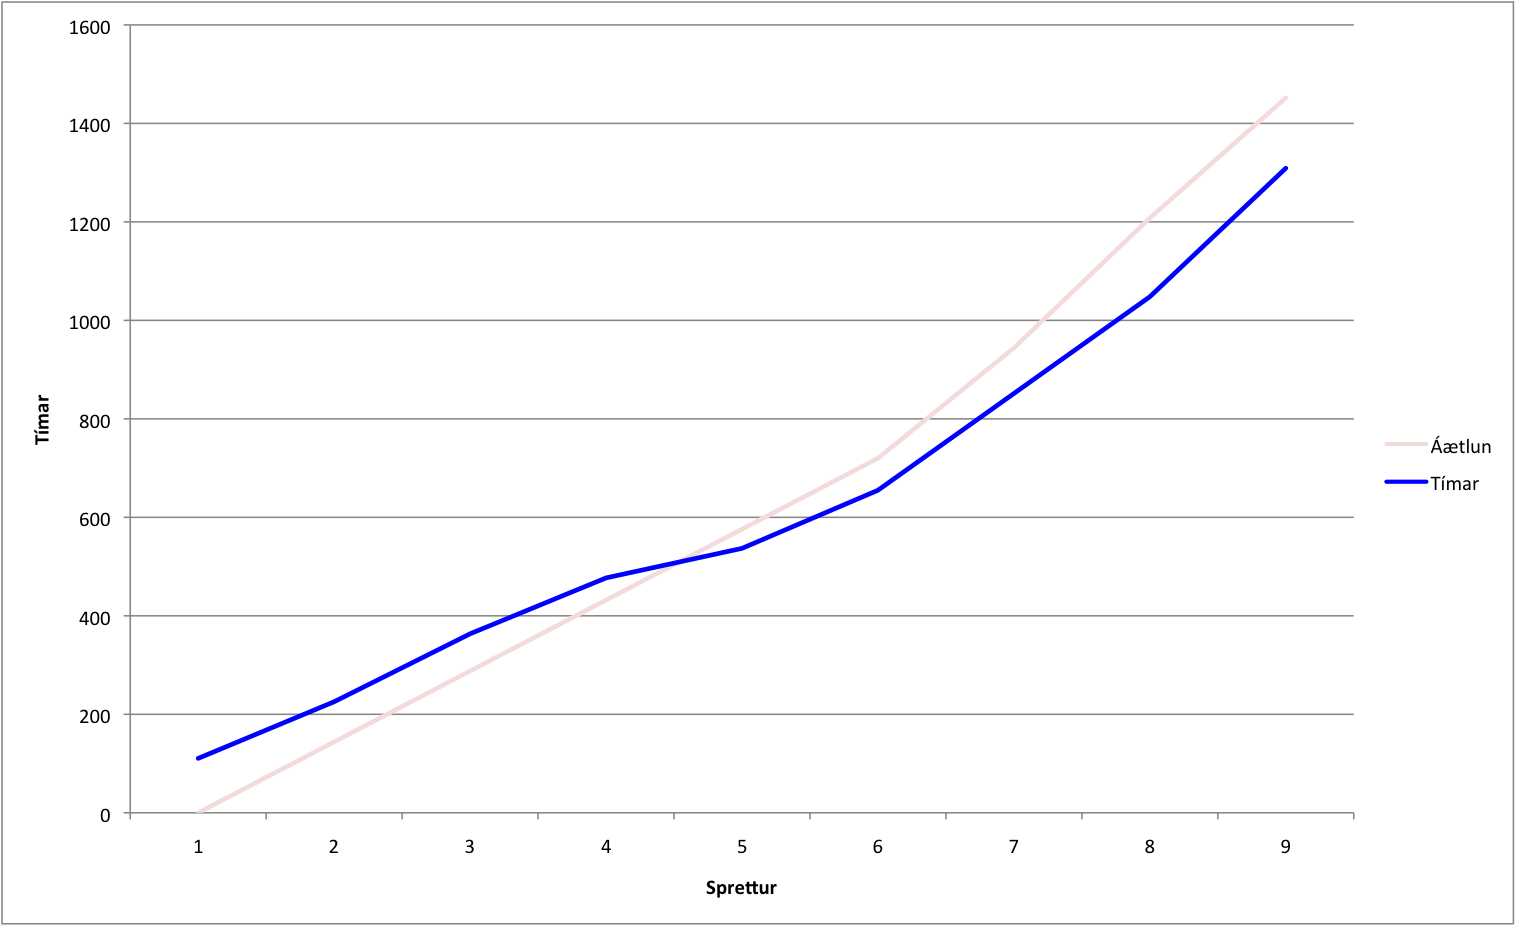
\includegraphics[width=1\textwidth]{fjoldi_vinnustunda.png} 
  \caption{fjöldi vinnustunda} 
\end{figure}

Taka ber fram að tímaáætlarnir okkar miðuðust við fyrsta til áttunda sprett og sýnir því grafið ekki þá tíma sem unnir voru í undirbúningi verkefnisins á haustönn 2010 sem og í spretti 0.

Hægt er að sjá nánari útlistingu á hvernig tíma okkar var varið í Dagbok.pdf skjali á meðfylgjandi disk.

\end{document}